% -*- root: main.tex -*-
%-------------------------------------------------------------------------------
\chapterimage{chapter_head_6.pdf} 

%-------------------------------------------------------------------------------
\chapter{ROS 도구}

%-------------------------------------------------------------------------------
\section{ROS 도구 (RViz)}\index{ROS 도구 (RViz)}

ROS는 "로봇 운영체제 강좌 : ROS 명령어" 에서 설명한 커맨드형 명령어 이외에도 ROS 활용에 필요한 다양한 도구들이 존재한다. 이는 커맨드형 명령어와 상호보완하는 형태로 ROS 유저들에게는 필수적으로 알아둬야 할 부분이다.

ROS 도구로는 ROS 유저들이 개인적으로 공개한 툴까지 포함하여 상당히 많은 수가 있는데 그 중에서 이번 강좌에서는 1) 3차원 시각화를 돕는 RViz\footnote{ROS wiki, RViz, http://wiki.ros.org/rviz}\footnote{ROS wiki, RViz User Guide, http://wiki.ros.org/rviz/UserGuide}, 2) 데이터 로깅 툴인 rqt\_bag\footnote{ROS wiki, RQT Bag, http://wiki.ros.org/rqt\_bag}, 3) 데이터 플롯 툴인 rqt\_plot\footnote{ROS wiki, RQT Plot, http://wiki.ros.org/rqt\_plot}. 4) 노드간의 관계 및 메시지를 확인 가능한 rqt\_graph\footnote{ROS wiki, RQT Graph, http://wiki.ros.org/rqt\_graph} , 5) GUI 통합 툴인 rqt\footnote{ROS wiki, RQT, http://wiki.ros.org/rqt} 을 알아볼 것이다. 있다. 이들 툴들은 ros와의 직접적인 처리를 행하는 것은 아니지만 ROS를 이용한 프로그래밍에 매우 유용한 보조툴이다. 

특히, ROS Fuerte 버전부터는 RViz는 rqt 라는 이름으로 rqt\_bag, rqt\_plot, rqt\_graph 등과 함께 36가지 플러그인이 통폐합되어 종합 GUI 툴로써 사용 가능해졌다. 그뿐만 아니라 rqt는 QT로 개발되어 있기 때문에 유저들이 자유롭게 플러그인을 개발하여 추가할 수도 있어서 매우 편리하다. 이번 강좌에서는 아래의 내용에 대해서 알아보도록 하자.

\begin{itemize}[leftmargin=*]
\item RViz : 3D visualization tool / 3차원 시각화 툴
\item rqt\_bag : Logging and Visualization Sensor Data, rosbag gui tool / 메시지 기록 GUI 유틸리티
\item rqt\_plot : Data Plot Tool / 2차원 데이터 플롯 툴 
\item rqt\_graph : 노드 및 메시지간의 상관 관계를 그래프로 나타내는 툴
\item rqt : QT 기반의 ROS GUI 개발 툴
\end{itemize}

%-------------------------------------------------------------------------------
\subsection{RViz 개요 및 활용}\index{RViz 개요 및 활용}

RViz는 ROS의 3차원 시각화 툴이다. ROS 네트워크상의 데이터를 3차원으로 표시하는 것이 주요 목적으로 센서 데이터를 시각화하여 확인할 수 있다. 

예를들어, 레이저 레인지 파인더(LRF: Laser Range Finder)의 센서로부터의 장애물과의 거리값, Kinect 및 Xtion과 같은 3차원 거리 센서의 포인트 클라우드 데이터 (PCD: Point Cloud Data), 카메라로부터 취득한 컬러 이미지 값 등을 실시간으로 표시할 수 있다. 

또한, 사용자가 지정한 폴리곤을 이용하여 각종 표시를 지원하고 있다. 특히, Interactive Markers 를 이용하여 사용자 노드로부터의 명령 및 데이터를 수신하여 상호호환적인 움직을 나타낼 수도 있다. 더불어, XML로 URDF(Unified Robot Description Format) 을 작성하여 로봇을 3차원 모델로 표현하고, 각각의 모델은 자유도에 따라 이동 및 구동 가능하도록 할 수 있어서 시뮬레이션 및 실시간 제어에 확인용으로 사용가능하다.

그 이외에 필자가 작성한 패키지중 RViz를 이용하여 표시가능한것을 아래에 링크하였다. 참고하길 바란다.

\begin{figure}[h]
\centering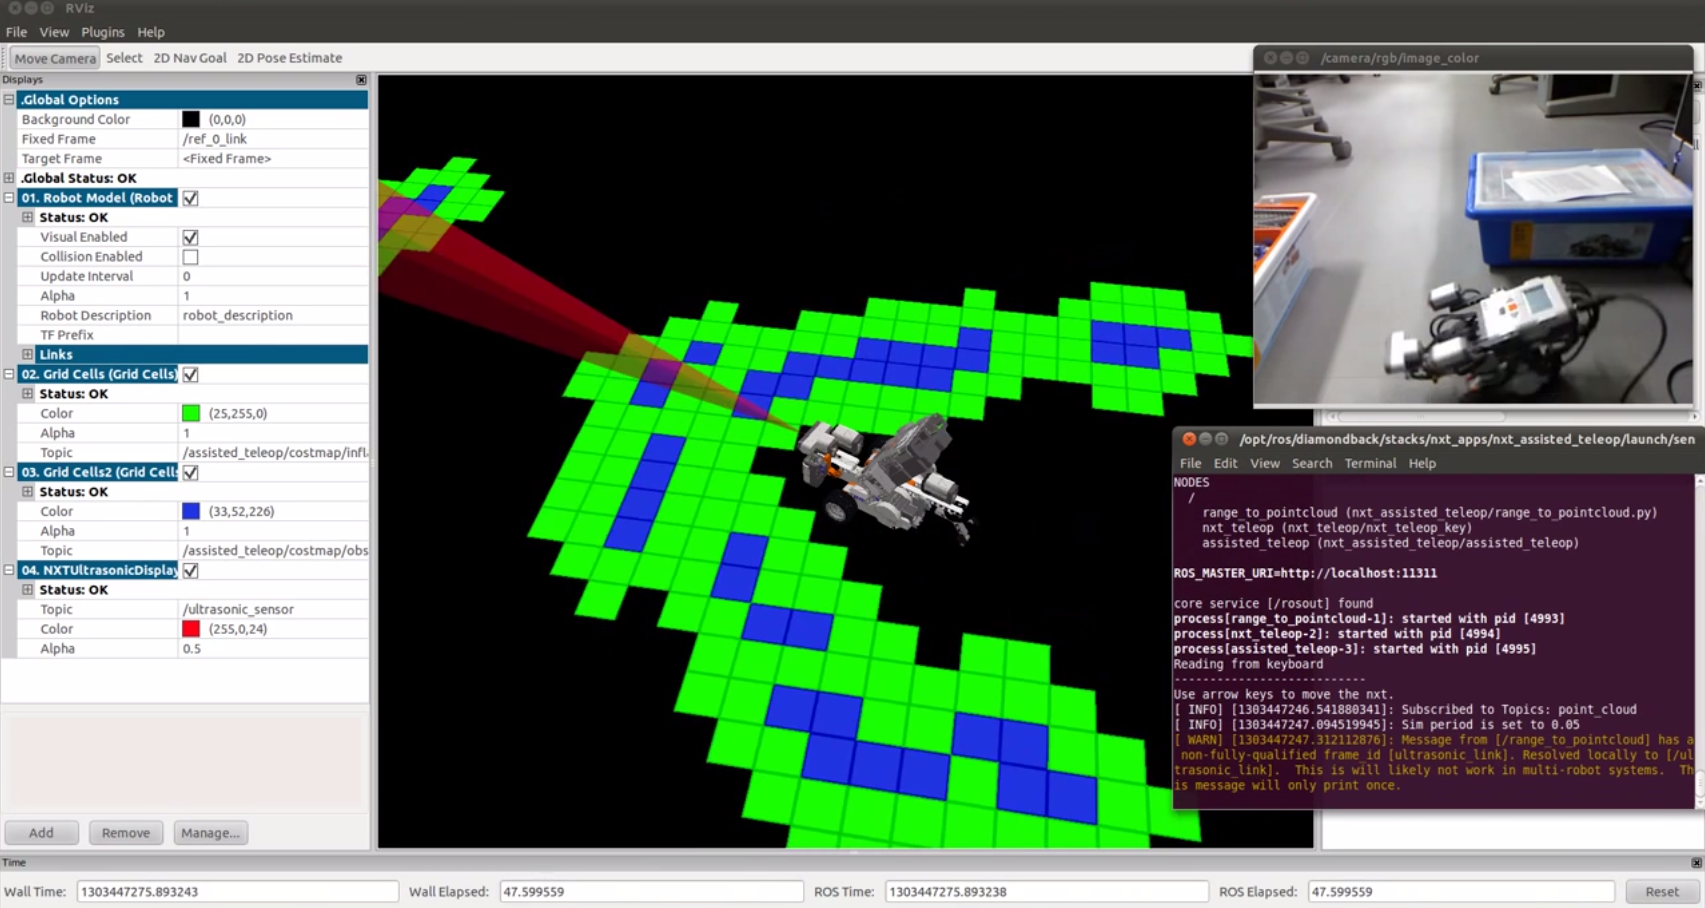
\includegraphics[width=0.7\columnwidth]{pictures/chapter6/rviz_example1.png}
\caption{RViz의 사용예1) 레고를 이용한 모바일 로봇과 초음파 센서를 이용하여 간단한 맵작성}
\end{figure}

\begin{figure}[h]
\centering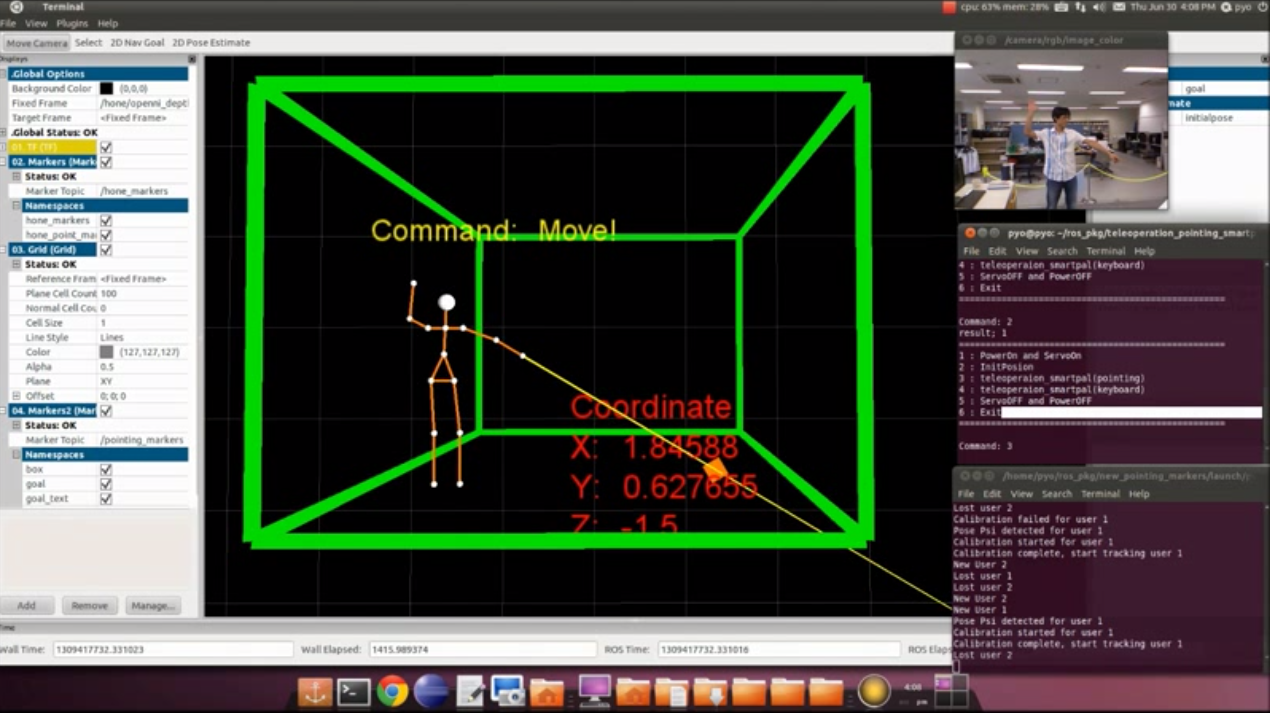
\includegraphics[width=0.7\columnwidth]{pictures/chapter6/rviz_example2.png}
\caption{RViz의 사용예2) 키넥트로부터 사람의 골격을 취득하고 로봇을 제어하는 모습}
\end{figure}

%-------------------------------------------------------------------------------
\subsection{RViz 설치 및 실행}\index{RViz 설치 및 실행}

ROS 설치시에 기본 설치라고도 부를 수 있는 "Desktop-Full Install" 를 설치하게되면 RViz는 기본적으로 설치되어 있다. 만약에 "Desktop-Full Install" 으로 설치하지 않았거나, RViz 가 설치되어 있지 않을 경우에는 아래의 명령어로 설치할 수있다.

\begin{lstlisting}[language=bash]
sudo apt-get install ros-indigo-rviz
\end{lstlisting}

\noindent
RViz 의 실행 명령어는 아래와 같다. (단, roscore 가 실행되어 있어야 한다.)

\begin{lstlisting}[language=bash]
rosrun rviz rviz
\end{lstlisting}

%-------------------------------------------------------------------------------
\subsection{RViz 화면 구성}\index{RViz 화면 구성}

\begin{figure}[h]
\centering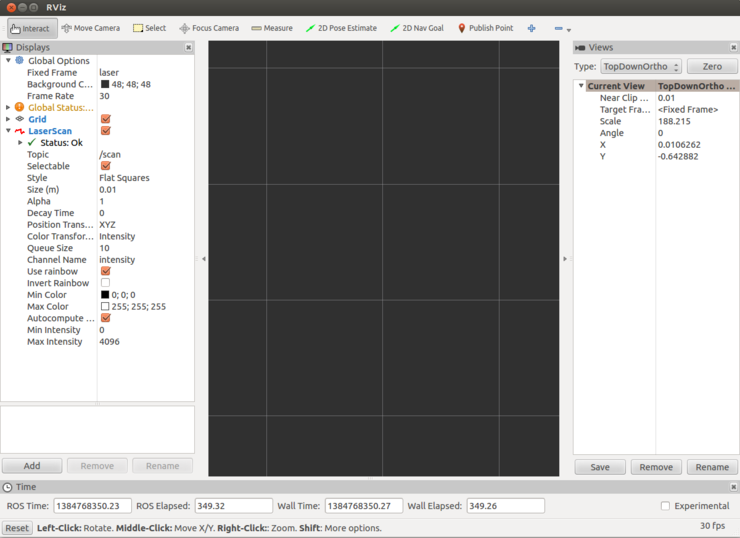
\includegraphics[width=0.8\columnwidth]{pictures/chapter6/rviz.png}
\caption{RViz 화면 구성}
\end{figure}

\begin{enumerate}[leftmargin=*, label=\arabic{*})]
\item 3D 뷰 (3D view)
: 위 화면의 가운데의 검정색 부분을 가르킨다. 각종 데이타를 3차원으로 볼 수 있는 메인 화면이다.

\item 디스플레이(Displays) 
: 왼쪽에 있는 디스플레이 화면은 각종 토픽으로부터 사용자가 원하는 데이타의 뷰를 선택하는 화면이다.

\item 메뉴 (Menu)
: 메뉴는 상단에 놓여져 있다. 현재의 뷰 상태를 저장하거나 읽어오는 명령, 각종 패널의 뷰 옵션을 체크할 수 있다.

\item 툴 (Tools)
: 대부분 네비게이션에 필요한 툴들이 놓여져 있다. 상세한 설명은 네비게이션을 다룰때 설명하도록 하겠다.

\item 뷰 (Views)
: 3D 뷰의 시점을 변경한다.

\item 시간 (Time)
: 현재 시간과 ROS Time 을 실시간으로 보여준다.
\end{enumerate}

%-------------------------------------------------------------------------------
% \subsection{사용 방법}\index{사용 방법}

%-------------------------------------------------------------------------------
\subsection{데이터 표시의 예}\index{데이터 표시의 예}

\begin{figure}[h]
\centering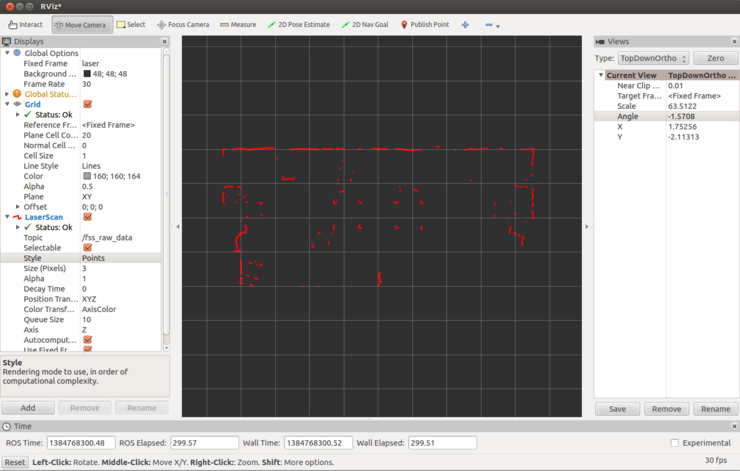
\includegraphics[width=0.7\columnwidth]{pictures/chapter6/rviz_example3.png}
\caption{RViz 사용예3) LRF를 이용한 거리측정}
\end{figure}

\begin{figure}[h]
\centering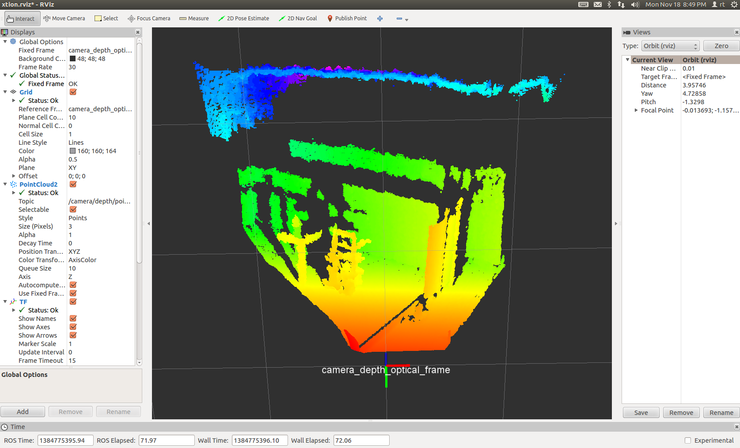
\includegraphics[width=0.7\columnwidth]{pictures/chapter6/rviz_example4.png}
\caption{RViz 사용예4) Xtion 센서로부터 취득한 3차원 거리 값}
\end{figure}

\begin{figure}[h]
\centering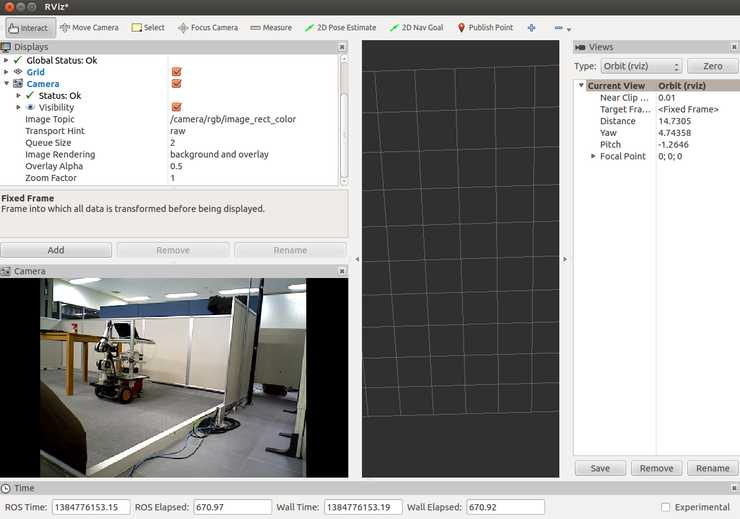
\includegraphics[width=0.7\columnwidth]{pictures/chapter6/rviz_example5.png}
\caption{RViz 사용예5) Xtion 센서에 장착된 카메라를 이용한 이미지 데이터 취득}
\end{figure}

%-------------------------------------------------------------------------------
\section{ROS 도구 (rqt) }\index{ROS 도구 (rqt) }

%-------------------------------------------------------------------------------
\subsection{rqt 개요}\index{rqt 개요}

ROS Fuerte 버전부터는 rqt 라는 이름으로 기존의 rxbag, rxplot, rxgraph 등이 통폐합되어 rqt\_bag, rqt\_plot, rqt\_graph 등을 플러그인으로 하는 종합 GUI 툴로써 사용 가능해졌다. 더불어, rviz 또한 rqt의 플러그인으로 편입되면서 rqt 는 ROS에서 빼놓을 수 없는 중요한 GUI 툴이 되었다. 그뿐만 아니라 rqt는 QT로 개발되어 있기 때문에 유저들이 자유롭게 플러그인을 개발하여 추가할 수도 있어서 매우 편리하다. 이번 강좌에서는 rqt의 대표적인 플러그인인 rqt\_bag, rqt\_plot, rqt\_graph 등 에 대해서 알아보도록 하겠다.

참고로, 그 이외에도 rqt\_action, rqt\_gui, rqt\_plot, rqt\_runtime\_monitorrqt\_bag, rqt\_gui\_cpp, rqt\_pose\_view, rqt\_rvizrqt\_bag\_plugins, rqt\_gui\_py, rqt\_publisher, rqt\_service\_callerrqt\_capabilities, rqt\_image\_view, rqt\_py\_common, rqt\_shellrqt\_console, rqt\_launch, rqt\_py\_console, rqt\_srvrqt\_controller\_manager, rqt\_logger\_level, rqt\_reconfigure, rqt\_tf\_treerqt\_dep, rqt\_moveit, rqt\_robot\_dashboard, rqt\_toprqt\_ez\_publisher, rqt\_msg, rqt\_robot\_monitor, rqt\_topicrqt\_graph, rqt\_nav\_view, rqt\_robot\_steering, rqt\_web 등의 플러그인이 존재한다.\sloppy

%-------------------------------------------------------------------------------
\subsection{rqt 설치}\index{rqt 설치}

ROS 설치시에 기본 설치라고도 부를 수 있는 "Desktop-Full Install" 를 설치하게되면 rqt는 기본적으로 설치되어 있다. 만약에 "Desktop-Full Install" 으로 설치하지 않았거나, rqt 가 설치되어 있지 않을 경우에는 아래의 명령어로 설치할 수있다.

\begin{lstlisting}[language=bash]
sudo apt-get install ros-indigo-rqt ros-indigo-rqt-common-plugins
\end{lstlisting}

추가로, rqt\_graph 에서는 그래프 생성을 위하여 추가적으로 설치해야할 파일이 있다. rqt\_graph 에서는 PyQtGraph, MatPlot, QwtPlot 을 지원하는데 우리는 rqt\_graph 가 추천하는 PyQtGraph 을 사용하도록 하자.

http://www.pyqtgraph.org/downloads/python-pyqtgraph\_0.9.8-1\_all.deb 에서 deb 파일을 받고 클릭하여 설치하도록 하자. 그 뒤 아래와 같이 rqt\_graph를 실행한 후, 프로그램의 오른쪽 상단에 있는 옵션을 의미하는 "기어" 모양의 아이콘을 클릭하면 아래의 첨부 그림과 같이 옵션을 선택할 수 있는데 PyQtGraph 를 선택해주면 된다. PyQtGraph 이외에도 MatPlot, QwtPlot 도 이용 가능하니 원하는 그래프 관련 라이브러리를 이용하면 된다.

\begin{lstlisting}[language=bash]
rqt_graph
\end{lstlisting}

\begin{figure}[h]
\centering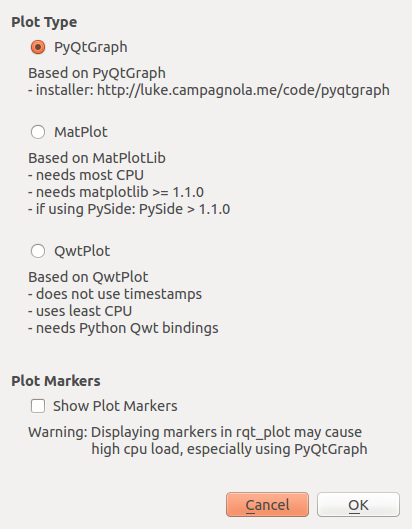
\includegraphics[width=0.5\columnwidth]{pictures/chapter6/rqtplotoption.png}
\caption{rqt\_graph의 설치 옵션}
\end{figure}

%-------------------------------------------------------------------------------
\subsection{rqt 실행 및 각 메뉴 소개}\index{rqt 실행 및 각 메뉴 소개}

실행은 아래와 같다. 단순히 rqt 라고 실행해주면 된다. (정식 실행명령어는 rosrun rqt\_gui rqt\_gui 이다)

\begin{lstlisting}[language=bash]
rqt
\end{lstlisting}

rqt 를 실행해주면 아래와 같이 rqt gui 화면이 나온다.처음 구동하였다면 아무런 표시가 없이 덩그러니 메뉴만 표시된다. 이는 rqt가 직접적으로 수행하는 프로그램인 플러그인이 지정되지 않았기 때문이다. 메뉴를 간단히 설명하자면, File의 경우, 단순히 rqt를 종료하는 서브메뉴만 있다. 플러그인(Plugins) 에는 27가지의 플러그인이 있다. 이를 선택하여 이용하게 된다. 동작(Running) 은 현재 동작중인 플러그인이 표시되어 필요치 않을시에 동작을 중단시킬 수 있는 메뉴이다. 끝으로 시각(Perspectives)은 현재 구동중인 플러그인을 셋트로 다음에도 같은 셋트를 이용하고 싶을때 저장하여 동일한 플러그인들을 실행할때 쓰는 메뉴이다.

\begin{figure}[h]
\centering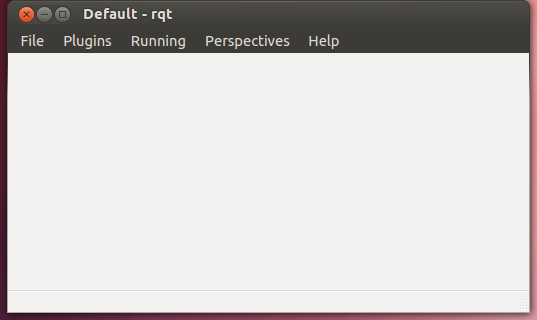
\includegraphics[width=0.6\columnwidth]{pictures/chapter6/rqt.png}
\caption{rqt의 초기 화면}
\end{figure}

%-------------------------------------------------------------------------------
\subsection{rqt 플러그인}\index{rqt 플러그인}

rqt의 상단 메뉴중에서 플러그인(Plugins)\footnote{ROS wiki, Plugins, http://wiki.ros.org/rqt/Plugins}\footnote{ROS wiki, RQT Common Plugins, http://wiki.ros.org/rqt\_common\_plugins}을 선택하면 27가지의 플러그인을 확인할 수 있다. 이 플러그인은 아래의 역할을 담당한다. 대부분 매우 필요한 기능등을 갖춘 rqt 의 기본 플러그인이다. 필요에 의해서 사용자가 개발한 플러그인도 추가 가능하다.

\subsubsection{액션 (Action)}
Action Type Browser | Action 타입의 데이터 구조를 확인하는 플러그인 
\subsubsection{구성 (Configuration)}
Dynamic Reconfigure | 노드들에서 제공하는 설정값 변경을 위한 GUI 설정값 변경 플러그인\\
Launch | roslaunch 의 GUI 플러그인, ROS런치의 이름 및 구성이 생각안날때 매우 유용하다.\\
\subsubsection{내성 (Introspection)}
Node Graph | 구동중인 모든 노드들의 관계도 및 메시지의 흐름을 확인할 수 있는 그래프 뷰 형식의 플러그인\\
Package Graph | 노드의 의존 관계를 표시하는 그래프 뷰 형식의 플러그인\\
Process Monitor | 현재 실행중인 노드들의 CPU사용률, 메모리사용륭, 스레드수 등을 확인 가능하다.\\
\subsubsection{로깅 (Logging)}
Bag | ROS 데이터 로깅 관련 플러그인\\
Console | 노드들에서 발생되는 경고(Warning), 에러(Error) 등의 메시지들을 한 화면에서 확인 가능한 플러그인\\
Logger Level | ROS의 Debug, Info, Warn, Error, Fatal 로거 정보를 선택하여 표시할 수 있는 GUI 툴\\
\subsubsection{다양한 툴 (Miscellaneous Tools)}
Python Console | 파이썬 콘솔 화면 플러그인\\
Shell | 쉘(shell)을 구동하는 플러그인\\
Web | 웹 브라우저를 구동하는 플러그인\\
\subsubsection{로봇 (Robot)}
사용하는 로봇에 따라 계기판(dashboard) 등의 플러그인을 이곳에 추가하면 된다. \\
\subsubsection{로봇툴 (Robot Tools)}
Controller Manager | 컨트롤러 제어에 필요한 플로그인\\
Diagnostic Viewer | 로봇 디바이스 및 에러 확인 플러그인\\
Moveit! Monitor | 로봇 팔 계획에 사용되는 Moveit! 데이터를 확인하는 플러그인\\
Robot Steering | 로봇 조정 GUI 툴, 원격 조정에서 이 GUI 툴을 이용하여 로봇 조종하기에 유용함.\\
Runtime Monitor | 실시간으로 노드들에서 발생되는 에러 및 경고를 확인가능한 플러그인\\
\subsubsection{서비스 (Services)}
Service Caller | 구동중인 서비스 서버에 접속하여 서비스를 요청하는 GUI 플러그인, 서비스 테스트에 유용하다.\\
Service Type Browser | 서비스 타입의 데이터 구조를 확인하는 플러그인\\
\subsubsection{토픽 (Topics)}
Easy Message Publisher | 토픽을 GUI 환경에서 발행가능 한 플러그인\\
Topic Publisher | 토픽을 생성하여 발행가능한 GUI 플러그인, 토픽 테스트에 매우 유용하다.\\
Topic Type Browser | 토픽 타입의 데이터 구조 확인 플러그인, 토픽 타입 확인에 매우 유용하다.\\
Topic Monitor | 현재 사용중인 토픽을 나열, 그 중에서 사용자가 선택한 토픽의 정보를 확인하는 플러그인\\
\subsubsection{시각화 (Visualization)}
Image View | 카메라의 영상 데이터를 확인 가능한 플러그인, 간단한 카메라 데이터 테스트에 유용하다.\\
Navigation Viewer | 로봇 네비게이션의 위치 및 목표지점 확인하는 플러그인\\
Plot | 2차원 데이터 플롯 GUI 플러그인, 2차원 데이터의 도식화에 매우 유용하다.\\
Pose View | 현재 tf의 위치 및 모델의 위치 표시 플러그인\\
RViz | 3차원 시각화 툴인 RViz 플러그인\\
TF Tree | tf 관계를 트리로 나타내는 그래프 뷰 형식의 플러그인\\

\begin{figure}[h]
\centering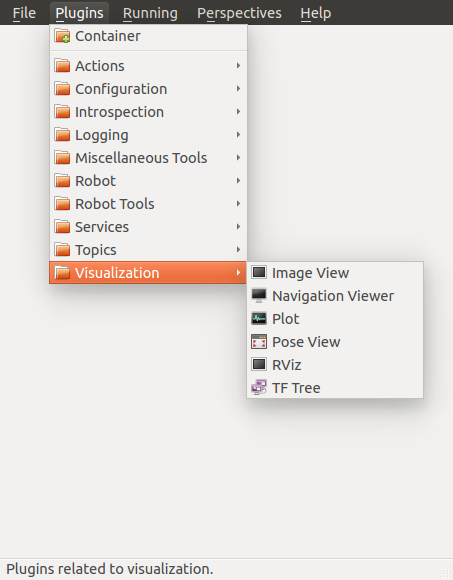
\includegraphics[width=0.8\columnwidth]{pictures/chapter6/rqt_plugin.png}
\caption{rqt 플러그인}
\end{figure}

\vspace{\baselineskip}
\noindent
이 들의 모든 플러그인을 설명하기 어렵고, 이번 강좌에서는 가장 빈번히 사용되는 rqt\_bag, rqt\_graph, rqt\_plot 등 에대해서 알아보도록 하겠다.

%-------------------------------------------------------------------------------
\subsection{rqt\_plot}\index{rqt\_plot}

rqt\_plot 은 2차원 데이터 플롯 툴이다. 플롯이라하면 좌료를 그리다라는 의미이다. 즉, ROS 메시지를 받아서 이를 좌표에 뿌리게 되는 것을 의미한다. 예를들어 turtlesim 노드 pose 메시지의 x 좌표와  y좌표를 좌표에 표기해보도록 하자. 우선, turtlesim 패키지의 turtlesim\_node 을 구동하자.

\begin{lstlisting}[language=ros]
$ rosrun turtlesim turtlesim_node 
\end{lstlisting}

다음으로, rqt\_plot 을 아래의 조건으로 구동하여 좌표를 작성한다. (원래는 rqt 를 구동후에 Plot 플러그인을 불러와서 GUI환경에서 토픽을 설정하면 되야하지만, 현재 버전에서는 이상하게 구동하지 않는다. 그러므로 아래의 명령어로 대채하여 설명한다.)

\begin{lstlisting}[language=ros]
rqt_plot /turtle1/pose/
\end{lstlisting}

다음으로, turtlesim 패키지의 turtle\_teleop\_key 을 구동하여, 화면속의 거북이를 이리저리 움직여보자.

\begin{lstlisting}[language=ros]
$ rosrun turtlesim turtle_teleop_key
\end{lstlisting}

그러면 빨간색 선이 거북이의 x위치가 x 좌표, 파란선이 거북이의 y위치가 y좌표에 표시됨을 확인할 수 있을 것이다. 이와 같이 2차원 데이터의 좌표 표시에 매우 유용한 툴로 지금은 turtlesim 을 이용하였지만, 사용자가 개발한 노드의 2차원 데이터 표시에 매우 유용할 것이다. 특히, 센서값 표시에 적합하다.

\begin{figure}[h]
\centering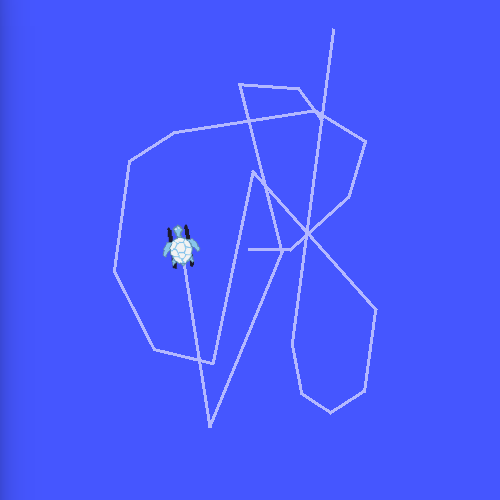
\includegraphics[height=50mm]{pictures/chapter6/turtlesim_rqt_plot1.png}
\centering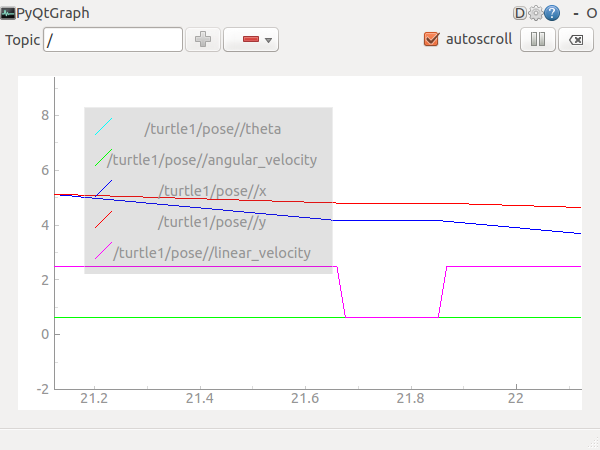
\includegraphics[height=50mm]{pictures/chapter6/turtlesim_rqt_plot2.png}
\caption{rqt\_plot 예제}
\end{figure}

%-------------------------------------------------------------------------------
\subsection{rqt\_bag}\index{rqt\_bag}

메시지 기록을 시각화한 GUI 툴이다. "로봇 운영체제 강좌 : ROS 정보 명령어 (rosbag)" 에서 다룬 내용을 시각화하면 편집 가능한 툴로 이미지 값등과 함께 편집할 때 매우 유용한 툴이다.

이를 테스트하기 위해서 위헤서 다룬 rqt\_graph 및 Image View 에서 다룬 turtlesim 및 uvc camera 관련의 노드들을 전부 실행해 주자. 그 뒤, 아래의 명령어로 카메라의 "/image\_raw" 와 터틀시뮬레이션의 "/turtle1/cmd\_vel" 값을 bag 파일로 생성하자.

\begin{lstlisting}[language=ros]
$ rosbag record /image_raw /turtle1/cmd_vel
\end{lstlisting}

그 후, 아래의 명령어로 rqt를 구동 후, 플러그인(Plugins) 메뉴에서 Bag를 선택한다. 그 뒤 왼쪽 상단의 폴더 모양(Load Bag)의 아이콘을 선택하여 방금전에 기록해둔 *.bag 파일을 불러오도록 하자. 그러면 아래의 화면처럼 영상 및 cmd\_vel 값을 확인할 수 있다. 또한, 이를 확대, 재생, 시간별 데이터 수 등을 확인할 수 있으며, 오른쪽 마우스를 누르면 Publish 라는 옵션이 있는데 이를 통해 메시지를 다시 발행할 수도 있다.

\begin{lstlisting}[language=ros]
$ rqt
\end{lstlisting}

\begin{figure}[h]
\centering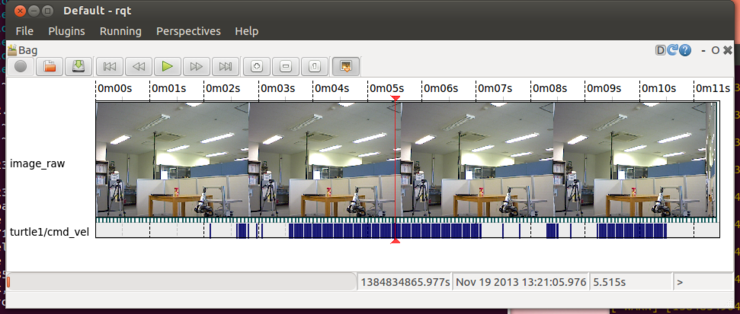
\includegraphics[width=0.9\columnwidth]{pictures/chapter6/rqt_bag.png}
\caption{rqtbag 예제}
\end{figure}

%-------------------------------------------------------------------------------
\subsection{rqt\_graph}\index{rqt\_graph}

현재 구동중인 노드 및 ROS 네트워크상에 전송되고 있는 메시지간의 상관 관계를 그래프로 나타내주는 툴이다. 현재 ROS 네트워크의 상황을 파악하는데에 매우 유용하다.

사용방법은 매우 간단한다. 아래의 명령어로 rqt를 구동후, 플러그인(Plugins) 메뉴에서 ROS Graph를 선택하면 그것으로 끝이다. 현재, 카메라 및 터틀봇시뮬레이션을 구동하셨을때의 노드 및 메시지의 상황은 아래 그림처럼 나타난다.

\begin{lstlisting}[language=ros]
$ rqt
\end{lstlisting}

\begin{figure}[h]
\centering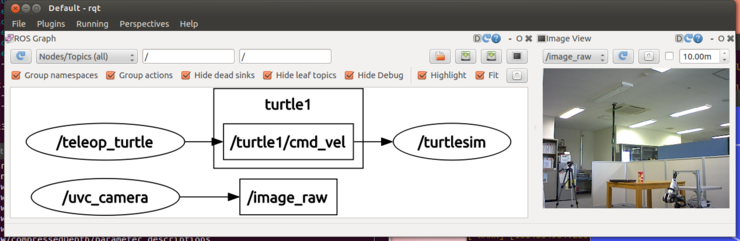
\includegraphics[width=0.9\columnwidth]{pictures/chapter6/rqt_graph.png}
\caption{rqt\_graph 예제}
\end{figure}

%-------------------------------------------------------------------------------
\subsection{Image View}\index{Image View}

카메라의 이미지 데이터를 표시하는 플러그인이다. 이미지 처리 프로세스는 아니지만, 단순히 영상을 확인하는 용도로는 매우 간단하기에 유용하다.

일반 USB CAM의 경우, UVC을 지원하기에 ROS의 "uvc\_camera"\footnote{ROS wiki, UVC Camera, http://wiki.ros.org/uvc\_camera} 패키지를 이용하면 된다. 우선, 아래의 명령어로 "uvc\_camera" 패키지를 설치하도록 하자.

\begin{lstlisting}[language=ROS]
$ sudo apt-get install ros-indigo-uvc-camera 
\end{lstlisting}

USB CAM을 컴퓨터의 USB에 연결하고, 아래의 명령어로 uvc\_camera 패키지의 uvc\_camera\_node 노드를 구동하자.

\begin{lstlisting}[language=ros]
$ rosrun uvc_camera uvc_camera_node
\end{lstlisting}

그 후, 아래의 명령어로 rqt를 구동후, 플러그인(Plugins) 메뉴에서 이미지 뷰(Image View)를 선택한다. 그 뒤 왼쪽 상단의 메시지 선택란을 "/image\_raw"를 선택하면 아래의 화면처럼 영상을 확인할 수 있다. 

\begin{lstlisting}[language=ros]
$ rqt
\end{lstlisting}

이상으로 rqt 를 대략적인 개요, 설치, 사용 방법에 대해서 설명하였다. 이 강좌를 통해서 모든 플러그인의 설명을 하는 것을 불가능했지만 위에서 설명한 몇가지 예를 기반으로 직접 사용해보기를 추천한다. ROS 노드와 같은 직접적으로 로봇 및 센서 처리에 관련한 내용은 아니지만, 이와 같은 작업들을 수행하는데 있어서 데이터를 저장, 보존, 수정, 현황파악 등에 도움이 되는 보조툴로서 사용가능하다. 













%-------------------------------------------------------------------------------